\subsection{Optimizations for LPA}
\label{sec:lpa}

We use a parallel implementation of LPA to determine suitable parameter settings and optimize the original algorithm through experimentation with a variety of techniques. We use \textit{asynchronous} version of LPA, where threads work independently on different parts of the graph. This allows for faster convergence but can also lead to more variability in the final result \cite{com-blondel08, com-halappanavar17}. Further, we allocate a separate hashtable per thread to keep track of the delta-modularity of moving to each community linked to a vertex in the local-moving phase of the algorithm, and to keep track of the total edge weight from one super-vertex to the other super-vertices in the aggregation phase of the algorithm.

Our optimizations include using OpenMP's \verb|dynamic| loop schedule, limiting the number of iterations per pass to $20$, using a tolerance drop rate of $10$, setting an initial tolerance of $0.01$, using an aggregation tolerance of $0.8$, employing vertex pruning, making use of parallel prefix sum and preallocated Compressed Sparse Row (CSR) data structures for finding community vertices and for storing the super-vertex graph during the aggregation phase, and using fast collision-free per-thread hashtables which are well separated in their memory addresses (\textit{Far-KV}) for the local-moving and aggregation phases of the algorithm. Details on each of the optimizations is given below.

For each optimization, we test a number of relevant alternatives, and show the relative time and the relative modularity of communities obtained by each alternative in Figure \ref{fig:rak-opt}. This result is obtained by running the tests on each graph in the dataset (see Table \ref{tab:dataset}), $5$ times on each graph to reduce the impact of noise, taking their geometric mean and arithmetic mean for the runtime and modularity respectively, and representing them as a ratio within each optimization category.


\subsubsection{Adjusting OpenMP loop schedule}

We attempt \textit{static}, \textit{dynamic}, \textit{guided}, and \textit{auto} loop scheduling approaches of OpenMP (each with a chunk size of $2048$) to parallelize the local-moving and aggregation phases of the Louvain algorithm. Results indicate that the scheduling behavior can have small impact on the quality of obtained communities. We consider OpenMP's \verb|dynamic| loop schedule to be the best choice, as it helps achieve better load balancing when the degree distribution of vertices is non-uniform, and offers a $7\%$ reduction in runtime with respect to OpenMP's \textit{auto} loop schedule, with only a $0.4\%$ reduction in the modularity of communities obtained (which is likely to be just noise).

\subsubsection{Limiting the number of iterations per pass}

Restricting the number of iterations of the local-moving phase ensures its termination within a reasonable number of iterations, which helps minimize runtime. This can be important since the local-moving phase performed in the first pass is the most expensive step of the algorithm. However, choosing too small a limit may worsen convergence rate. Our results indicate that limiting the maximum number of iterations to $20$ allows for $13\%$ faster convergence, when compared to a maximum iterations of $100$.


\subsubsection{Adjusting tolerance drop rate (threshold scaling)}

Tolerance is used to detect convergence in the local-moving phase of the Louvain algorithm, i.e., when the total delta-modularity in a given iteration is below or equal to the specified tolerance, the local-moving phase is considered to have converged. Instead of using a fixed tolerance across all passes of the Louvain algorithm, we can start with an initial high tolerance and then gradually reduce it. This is known as threshold scaling \cite{com-lu15, com-naim17, com-halappanavar17}, and it helps minimize runtime as the first pass of the algorithm (which is usually the most expensive). Based on our findings, a tolerance drop rate of $10$ yields $4\%$ faster convergence, with respect to a tolerance drop rate of $1$ (threshold scaling disabled), with no reduction in quality of communities obtained.


\subsubsection{Adjusting initial tolerance}

Starting with a smaller initial tolerance allows the algorithm to explore broader possibilities for community assignments in the early stage, but comes at the cost of increased runtime. We find an initial tolerance of $0.01$ provides a $14\%$ reduction in runtime of the algorithm with no reduction in the quality of identified communities, when compared to an initial tolerance of $10^{-6}$.


\subsubsection{Adjusting aggregation tolerance}

The aggregation tolerance determines the point at which communities are considered to have converged based on the number of community merges. In other words, if too few communities merged this pass we should stop here, i.e., if $|V_{aggregated}|/|V| \geq$ aggregation tolerance, we consider the algorithm to have converged. Adjusting aggregation tolerance allows the algorithm to stop earlier when further merges have minimal impact on the final result. According to our observations, an aggregation tolerance of $0.8$ appears to be the best choice, as it presents a $14\%$ reduction in runtime, when compared to the aggregation tolerance being disabled ($1$), while identifying final communities of equivalent quality.


\subsubsection{Vertex pruning}

Vertex pruning is a technique that is used to minimize unnecessary computation. Here, when a vertex changes its community, its marks its neighbors to be processed. Once a vertex has been processed, it is marked as not to be processed. However, it comes with an added overhead of marking an unmarking of vertices. Based on our results, vertex pruning justifies this overhead, and should be enabled for $11\%$ improvement in performance. An illustration of vertex pruning optimization is shown in Figure \ref{fig:rak-pruning}.

\begin{figure}[hbtp]
  \centering
  \subfigure{
    \label{fig:rak-pruning--all}
    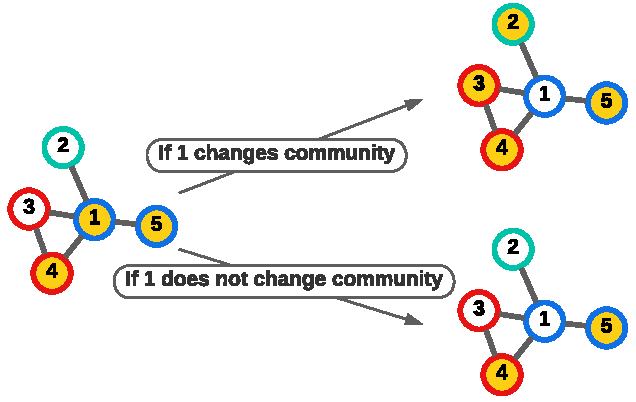
\includegraphics[width=0.78\linewidth]{out/rak-pruning.pdf}
  } \\[-2ex]
  \caption{Illustration of vertex pruning optimization: After processing vertex $1$, it's unmarked. If vertex $1$ changes its community, its neighbors are marked for processing. Community membership of each vertex is depicted by border color, and marked vertices are highlighted in yellow \cite{sahu2023gvelouvain}.}
  \label{fig:rak-pruning}
\end{figure}



\subsubsection{Finding community vertices for aggregation phase}

In the aggregation phase of the Louvain algorithm, the communities obtained in the previous local-moving phase of the algorithm are combined into super-vertices in the aggregated graph, with the edges between two super-vertices being equal to the total weight of edges between the respective communities. This requires one to obtain the list of vertices belonging to each community, instead of the mapping of community membership of each vertex that we have after the local-moving phase ends. A straight-forward implementation of this would make use of two-dimensional arrays for storing vertices belonging to each community, with the index in the first dimension representing the community id $c$, and the index in the second dimension pointing to the $n^{th}$ vertex in the given community $c$. However, this requires memory allocation during the algorithm, which is expensive. Employing a parallel prefix sum technique along with a preallocated Compressed Sparse Row (CSR) data structure eliminates repeated memory allocation and deallocation, enhancing performance. Indeed, out findings indicate that using parallel prefix sum along with a preallocated CSR is $2.2\times$ faster than using 2D arrays for aggregating vertices.


\subsubsection{Storing aggregated communities (super-vertex graph)}

After the list of vertices belonging to each community have been obtained, the communities need to be aggregated (or compressed) into super-vertices, such that edges between two super-vertices being equal to the total weight of edges between the respective communities. This is generally called the super-vertex graph, or the compressed graph. It is then used as an input to the local-moving phase of the next pass of the Louvain algorithm. A simple data structure to store the super-vertex graph in the adjacency list format would be a two-dimensional array. Again, this requires memory allocation during the algorithm, which is bad for performance. Utilizing two preallocated CSRs, one for the source graph and the other for the target graph (except the first pass, where the dynamic graph may be stored in any desired format suitable for dynamic batch updates), along with parallel prefix sum can help here. We observe that using parallel prefix sum along with preallocated CSRs for maintaining the super-vertex graph is again $2.2\times$ faster than using 2D arrays.


\subsubsection{Hashtable design for local-moving/aggregation phases}

One can use C++'s inbuilt maps as per-thread (independent) hashtables for the Louvain algorithm. But this has poor performance. So we use a key-list and a full-size values array (collision-free) to dramatically improve performance. However, if the memory addresses of the hashtables are nearby (\textit{Close-KV}), even if each thread uses its own hashtable exclusively, performance is not as high. This is possibly due to false cache-sharing. Alternatively, if we ensure that the memory address of each hashtable are farther away (\textit{Far-KV}), the performance improves. Our results indicate that \textit{Far-KV} has the best performance and is $4.4\times$ faster than \textit{Map}, and $1.3\times$ faster than \textit{Close-KV} hashtable implementations. An illustration of \textit{Far-KV} hashtable is shown in Figure \ref{fig:rak-hashtable}.

\begin{figure}[hbtp]
  \centering
  \subfigure{
    \label{fig:rak-hashtable--all}
    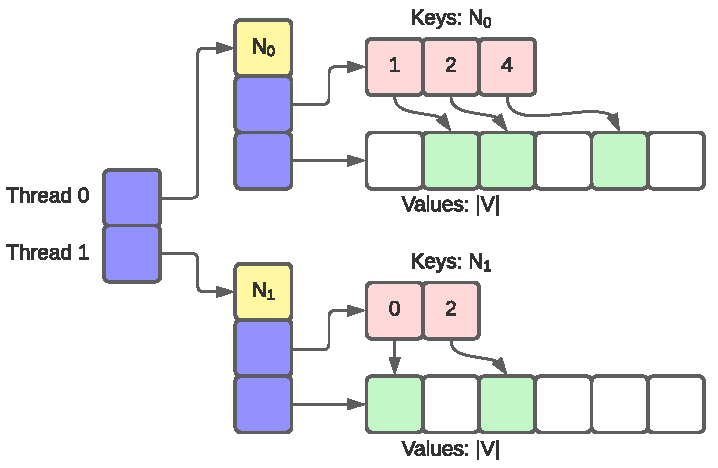
\includegraphics[width=0.88\linewidth]{out/rak-hashtable.pdf}
  } \\[-2ex]
  \caption{Illustration of collision-free per-thread hashtables that are well separated in their memory addresses (Far-KV), for two threads. Each hashtable consists of a keys vector, values vector (of size $|V|$), and a key count ($N_0$/$N_1$). The value associated with each key is stored/accumulated in the index pointed by the key. As the key count of each hashtable is updated independently, we allocate it separately on the heap to avoid false cache sharing \cite{sahu2023gvelouvain}.}
  \label{fig:rak-hashtable}
\end{figure}

\begin{figure*}[hbtp]
  \centering
  \subfigure{
    \label{fig:rak-opt--all}
    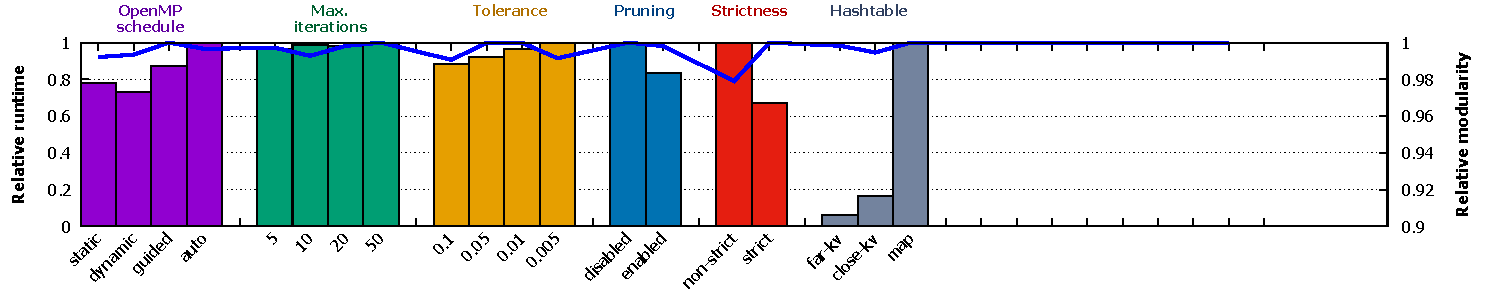
\includegraphics[width=0.98\linewidth]{out/rak-opt.pdf}
  } \\[-2ex]
  \caption{Impact of\ignore{various} parameter controls and optimizations on the runtime and result quality (modularity) of LPA. We show the impact of each optimization upon the relative runtime on the left Y-axis, and upon the relative modularity on the right Y-axis.}
  \label{fig:rak-opt}
\end{figure*}





\subsection{Our optimized LPA implementation}

We now explain the implementation of GVE-LPA in Algorithms \ref{alg:rak}, \ref{alg:raklm}, and \ref{alg:rakag}.


\subsubsection{Main step of GVE-LPA}

The main step of GVE-Louvain (\texttt{louvian()} function) is outlined in Algorithm \ref{alg:rak}. It encompasses initialization, the local-moving phase, and the aggregation phase. Here, the \texttt{louvain()} function takes the input graph $G$, and returns the community membership $C$ for each vertex. In line \ref{alg:louvain--initialization}, we first initializes the community membership $C$ of each vertex in $G$, and perform passes of the Louvain algorithm, limited to $MAX\_PASSES$ (lines \ref{alg:louvain--passes-begin}-\ref{alg:louvain--passes-end}). In each pass, we initialize the total edge weight of each vertex $K'$, the total edge weight of each community $\Sigma'$, and the community membership $C'$ of each vertex in the current graph $G'$ (line \ref{alg:louvain--reset-weights}); and mark all vertices as unprocessed (line \ref{alg:louvain--reset-affected}).

Next, in line \ref{alg:louvain--local-move}, we perform the local-moving phase by calling \texttt{louvainMove()} (Algorithm $\ref{alg:louvainlm}$), which optimizes community assignments. If the local-moving phase converged in a single iteration, global convergence is implied and we terminate the passes (line \ref{alg:louvain--globally-converged}). Further, if the drop is community count $|\Gamma|$ is too small, we have reached the point of diminishing returns, and thus stop at the current pass (line \ref{alg:louvain--aggregation-tolerance}).

In case convergence has not been achieved, we renumber communities (line \ref{alg:louvain--renumber}), update top-level community memberships $C$ with dendrogram lookup (line \ref{alg:louvain--lookup}), perform the aggregation phase by calling \texttt{louvainAggregate()} (Algorithm \ref{alg:louvainag}), and scale the convergence threshold for subsequent passes, i.e., perform threshold scaling (line \ref{alg:louvain--threshold-scaling}). The next pass continues in line \ref{alg:louvain--passes-begin}. At the end of all passes, we perform a final update of the top-level community memberships $C$ with dendrogram lookup (line \ref{alg:louvain--lookup-last}), and return the top-level community membership $C$ of each vertex in $G$.

\begin{algorithm}[hbtp]
\caption{GVE-LPA: Our parallel Label Propagation Algorithm (LPA).}
\label{alg:rak}
\begin{algorithmic}[1]
\Require{$G'$: Input graph}
\Require{$C$: Community membership of each vertex}
\Require{$G'$: Input/super-vertex graph}
\Require{$C'$: Community membership of each vertex in $G'$}
\Require{$K'$: Total edge weight of each vertex}
\Require{$\Sigma'$: Total edge weight of each community}
\Ensure{$G'_{C'}$: Community vertices (CSR)}
\Ensure{$H_t$: Collision-free per-thread hashtable}
\Ensure{$l_i$: Number of iterations performed (per pass)}
\Ensure{$l_p$: Number of passes performed}
\Ensure{$\tau$: Per iteration tolerance}
\Ensure{$\tau_{agg}$: Aggregation tolerance}

\Statex

\Function{louvain}{$G$} \label{alg:louvain--begin}
  \State Vertex membership: $C \gets [0 .. |V|)$ \textbf{;} $G' \gets G$ \label{alg:louvain--initialization}
  \ForAll{$l_p \in [0 .. \text{\small{MAX\_PASSES}})$} \label{alg:louvain--passes-begin}
    \State $\Sigma' \gets K' \gets vertexWeights(G')$ \textbf{;} $C' \gets [0 .. |V'|)$ \label{alg:louvain--reset-weights}
    \State Mark all vertices in $G'$ as unprocessed \label{alg:louvain--reset-affected}
    \State $l_i \gets louvainMove(G', C', K', \Sigma')$ \label{alg:louvain--local-move}
    \If{$l_i \le 1$} \textbf{break} \Comment{Globally converged?} \label{alg:louvain--globally-converged}
    \EndIf
    \State $|\Gamma|, |\Gamma_{old}| \gets$ Number of communities in $C$, $C'$
    \If{$|\Gamma|/|\Gamma_{old}| > \tau_{agg}$} \textbf{break} \Comment{Low shrink?} \label{alg:louvain--aggregation-tolerance}
    \EndIf
    \State $C' \gets$ Renumber communities in $C'$ \label{alg:louvain--renumber}
    \State $C \gets$ Lookup dendrogram using $C$ to $C'$ \label{alg:louvain--lookup}
    \State $G' \gets louvainAggregate(G', C')$ \label{alg:louvain--aggregate}
    \State $\tau \gets \tau / \text{\small{TOLERANCE\_DROP}}$ \Comment{Threshold scaling} \label{alg:louvain--threshold-scaling}
  \EndFor \label{alg:louvain--passes-end}
  \State $C \gets$ Lookup dendrogram using $C$ to $C'$ \label{alg:louvain--lookup-last}
  \Return{$C$} \label{alg:louvain--return}
\EndFunction \label{alg:louvain--end}
\end{algorithmic}
\end{algorithm}

\begin{algorithm}[hbtp]
\caption{Local-moving phase of GVE-Louvain.}
\label{alg:louvainlm}
\begin{algorithmic}[1]
\Require{$G'$: Input/super-vertex graph}
\Require{$C'$: Community membership of each vertex}
\Require{$K'$: Total edge weight of each vertex}
\Require{$\Sigma'$: Total edge weight of each community}
\Ensure{$G'_{C'}$: Community vertices (CSR)}
\Ensure{$H_t$: Collision-free per-thread hashtable}
\Ensure{$l_i$: Number of iterations performed}
\Ensure{$\tau$: Per iteration tolerance}

\Statex

\Function{louvainMove}{$G', C', K', \Sigma'$} \label{alg:louvainlm--move-begin}
  \ForAll{$l_i \in [0 .. \text{\small{MAX\_ITERATIONS}})$} \label{alg:louvainlm--iterations-begin}
    \State Total delta-modularity per iteration: $\Delta Q \gets 0$ \label{alg:louvainlm--init-deltaq}
    \ForAll{unprocessed $i \in V'$ \textbf{in parallel}} \label{alg:louvainlm--loop-vertices-begin}
      \State Mark $i$ as processed (prune) \label{alg:louvainlm--prune}
      \State $H_t \gets scanCommunities(\{\}, G', C', i, false)$ \label{alg:louvainlm--scan}
      \State $\rhd$ Use $H_t, K', \Sigma'$ to choose best community
      \State $c^* \gets$ Best community linked to $i$ in $G'$ \label{alg:louvainlm--best-community-begin}
      \State $\delta Q^* \gets$ Delta-modularity of moving $i$ to $c^*$ \label{alg:louvainlm--best-community-end}
      \If{$c^* = C'[i]$} \textbf{continue} \label{alg:louvainlm--best-community-same}
      \EndIf
      \State $\Sigma'[C'[i]] -= K'[i]$ \textbf{;} $\Sigma'[c^*] += K'[i]$ \textbf{atomic} \label{alg:louvainlm--perform-move-begin}
      \State $C'[i] \gets c^*$ \textbf{;} $\Delta Q \gets \Delta Q + \delta Q^*$ \label{alg:louvainlm--perform-move-end}
      \State Mark neighbors of $i$ as unprocessed \label{alg:louvainlm--remark}
    \EndFor \label{alg:louvainlm--loop-vertices-end}
    \If{$\Delta Q \le \tau$} \textbf{break} \Comment{Locally converged?} \label{alg:louvainlm--locally-converged}
    \EndIf
  \EndFor \label{alg:louvainlm--iterations-end}
  \Return{$l_i$} \label{alg:louvainlm--return}
\EndFunction \label{alg:louvainlm--move-end}

\Statex

\Function{scanCommunities}{$H_t, G', C', i, self$}
  \ForAll{$(j, w) \in G'.edges(i)$}
    \If{$self$ \textbf{or} $i \neq j$} $H_t \gets H_t[C'[j]] + w$
    \EndIf
  \EndFor
  \Return{$H_t$}
\EndFunction
\end{algorithmic}
\end{algorithm}

\begin{algorithm}[hbtp]
\caption{Aggregation phase of GVE-Louvain.}
\label{alg:louvainag}
\begin{algorithmic}[1]
\Require{$G'$: Input/super-vertex graph}
\Require{$C'$: Community membership of each vertex}
\Ensure{$G'_{C'}$: Community vertices (CSR)}
\Ensure{$G''$: Super-vertex graph (weighted CSR)}
\Ensure{$*.offsets$: Offsets array of a CSR graph}
\Ensure{$H_t$: Collision-free per-thread hashtable}

\Statex

\Function{louvainAggregate}{$G', C'$}
  \State $\rhd$ Obtain vertices belonging to each community
  \State $G'_{C'}.offsets \gets countCommunityVertices(G', C')$ \label{alg:louvainag--coff-begin}
  \State $G'_{C'}.offsets \gets exclusiveScan(G'_{C'}.offsets)$ \label{alg:louvainag--coff-end}
  \ForAll{$i \in V'$ \textbf{in parallel}} \label{alg:louvainag--comv-begin}
    \State Add edge $(C'[i], i)$ to CSR $G'_{C'}$ atomically
  \EndFor \label{alg:louvainag--comv-end}
  \State $\rhd$ Obtain super-vertex graph
  \State $G''.offsets \gets communityTotalDegree(G', C')$ \label{alg:louvainag--yoff-begin}
  \State $G''.offsets \gets exclusiveScan(G''.offsets)$ \label{alg:louvainag--yoff-end}
  \State $|\Gamma| \gets$ Number of communities in $C'$
  \ForAll{$c \in [0, |\Gamma|)$ \textbf{in parallel}} \label{alg:louvainag--y-begin}
    \If{degree of $c$ in $G'_{C'} = 0$} \textbf{continue}
    \EndIf
    \State $H_t \gets \{\}$
    \ForAll{$i \in G'_{C'}.edges(c)$}
      \State $H_t \gets scanCommunities(H, G', C', i, true)$
    \EndFor
    \ForAll{$(d, w) \in H_t$}
      \State Add edge $(c, d, w)$ to CSR $G''$ atomically
    \EndFor
  \EndFor \label{alg:louvainag--y-end}
  \Return $G''$ \label{alg:louvainag--return}
\EndFunction
\end{algorithmic}
\end{algorithm}



\subsubsection{Local-moving phase of GVE-Louvain}

The pseuodocode for the local-moving phase of GVE-Louvain is presented in Algorithm \ref{alg:louvainlm}, which iteratively moves vertices between communities to maximize modularity. Here, the \texttt{louvainMove()} function takes the current graph $G'$, community membership $C'$, total edge weight of each vertex $K'$, and total edge weight of each community $\Sigma'$ as input, and returns the number of iterations performed $l_i$.

Lines \ref{alg:louvainlm--iterations-begin}-\ref{alg:louvainlm--iterations-end} represent the main loop of the local-moving phase. In line \ref{alg:louvainlm--init-deltaq}, we first initialize the total delta-modularity per iteration $\Delta Q$. Next, in lines \ref{alg:louvainlm--loop-vertices-end}-\ref{alg:louvainlm--loop-vertices-end}, we iterate over unprocessed vertices in parallel. For each vertex $i$, we mark $i$ as processed - vertex pruning (line \ref{alg:louvainlm--prune}), scan communities connected to $i$ - excluding self (line \ref{alg:louvainlm--scan}), determine the best community $c*$ to move $i$ to (line \ref{alg:louvainlm--best-community-begin}), calculate the delta-modularity of moving $i$ to $c*$ (line \ref{alg:louvainlm--best-community-end}), and update the community membership  (lines \ref{alg:louvainlm--perform-move-begin}-\ref{alg:louvainlm--perform-move-end}) of $i$, and mark its neighbors as unprocessed (line \ref{alg:louvainlm--remark}) if a better community was found. In line \ref{alg:louvainlm--locally-converged}, we check if the local-moving phase has converged (locally). If so, we break out of the loop (or if $MAX\_ITERATIONS$ is reached). At the end, in line \ref{alg:louvainlm--return}, we return the number of iterations performed $l_i$.


\subsubsection{Aggregation phase of GVE-Louvain}

Finally, the psuedocode for the aggregation phase is shown in Algorithm \ref{alg:louvainag}, which aggregates communities into super-vertices. Here, the \texttt{louvainAggrega} \texttt{te()} function takes the current graph $G'$ and the community membership $C'$ as input, and returns the super-vertex graph $G''$.

In lines \ref{alg:louvainag--coff-begin}-\ref{alg:louvainag--coff-end}, the offsets array for the community vertices CSR $G'_{C'}.offsets$ is obtained by first counting the number of vertices belonging to each community using \texttt{countCommunity} \texttt{Vertices()}, and then performing exclusive scan on the array. In lines \ref{alg:louvainag--comv-begin}-\ref{alg:louvainag--comv-end}, we iterate over all vertices in parallel and atomically populate vertices belonging to each community into the community graph CSR $G'_{C'}$. Next, we obtain the offsets array for the super-vertex graph CSR by over-estimating the degree of each super-vertex, i.e., by obtaining the total degree of each community with \texttt{communityTotalDegree()}, and then performing exclusive scan on the array (lines \ref{alg:louvainag--yoff-begin}-\ref{alg:louvainag--yoff-end}). This causes the super-vertex graph CSR to be holey, i.e., with gaps in between the edges and weights array of each super-vertex in the CSR. Then, in lines \ref{alg:louvainag--y-begin}-\ref{alg:louvainag--y-end}, we iterate over all communities $c \in [0, |\Gamma|)$ in parallel, and add all communities $d$ (with associated edge weight $w$) linked to each vertex $i$ belonging to community $c$ (with \texttt{scanCommunities()} defined in Algorithm \ref{alg:louvainlm}) to the per-thread hashtable $H_t$. Once $H_t$ is populated with all communities (and associated weights) linked to community $c$, we add them as edges to super-vertex $c$ into the super-vertex graph $G''$ atomically. At the end, in line \ref{alg:louvainag--return}, we return the super-vertex graph $G''$.

\ignore{The main Louvain algorithm, given in Algorithm \ref{alg:louvain} first initializes the community membership of each vertex. It then iteratively performs the local-moving phase until convergence. In each pass, it resets the edge weights, marks vertices as unprocessed, and performs the local-moving phase. If the algorithm globally converges or the communities' shrinkage is below a specified tolerance, it breaks the loop. Otherwise, it renumbers the communities, updates the graph, and adjusts the convergence threshold. The main algorithm returns the final community membership of each vertex.}

\ignore{The local-moving phase is responsible for iteratively moving vertices between communities to maximize modularity. It uses a per-thread hashtable to keep track of the communities and their weights. The algorithm iterates over unprocessed vertices, scans their neighbors, and identifies the best community for each vertex based on delta-modularity. If the best community is different from the current community, it updates the community memberships and marks neighbors as unprocessed. The process continues until a specified number of iterations or until local convergence is achieved.}

\ignore{The aggregation phase aggregates communities into super-vertices to reduce the size of the graph. It first counts the vertices in each community and constructs a new graph with community vertices. It then calculates the total degree of each community and constructs a super-vertex graph. The algorithm ensures that only communities with a non-zero degree are considered. It utilizes a per-thread hashtable to efficiently aggregate edges between communities. The resulting super-vertex graph is returned to the main algorithm for the next iteration.}
